\section{Spatial Coupling: Supplementary Results}
\label{sec:appendix-spatial}

This section supplements the implementation details and additional results for \S\ref{sec:eval-spatial}, including triage strategy definitions and their combinations, the complete numerical results and interpretation of the window-width $W$ ablation, and halo suppression analysis.


\subsection{Derivation Details for the Candidate-Set Size Expectation}
\label{sec:appendix-candidate-expectation}

This section provides the detailed derivation behind Equations~\eqref{eq:cand-expectation} and~\eqref{eq:halo-prob} in the main text. Consider the section axis of a single view as a linear interval (without circular wrap-around), with window width~$W$ and window start positions approximately uniform over $[1,\,L{-}W{+}1]$. If signals are separable, the top-$t$ truncation covers the high-energy windows of all dirty segments. A clean segment is falsely included in the candidate set in a single view if and only if its window overlaps on the section axis with any selected window. For two windows of width~$W$, overlap occurs if and only if their start positions differ by less than~$W$; each selected window therefore ``contaminates'' a neighborhood of width $2W{-}1$ on the section axis.

When $t(2W{-}1)\ll L$ so that these contaminated neighborhoods are approximately non-overlapping, the probability that a clean segment's window start falls within a contaminated region is
\[
p_{\mathrm{halo}} \approx \frac{t(2W{-}1)}{L},
\]
which is Equation~\eqref{eq:halo-prob} in the main text. After intersecting candidate sets across $V$ approximately independent views, the probability that a clean segment is falsely included in every view is approximately $p_{\mathrm{halo}}^V$; multiplying by the total number of clean segments $P{-}B$ gives the expected false-inclusion volume, while the contribution from truly dirty segments is~$B$, yielding Equation~\eqref{eq:cand-expectation}.

\subsection{Break-Even Condition for $W$}
\label{sec:appendix-w-pricing}

The preceding section established the relationship between $p_{\mathrm{halo}}$ and $(t, W, L)$. In practice, $t$ is not a free parameter but is determined by the minimum truncation count $t_{\mathrm{op}}(W)$ required for target recall. Substituting into Equation~\eqref{eq:halo-prob} gives the operating false-inclusion probability
\begin{equation*}
p_{\mathrm{halo,op}}(W)
\;\triangleq\;
p_{\mathrm{halo}}\!\bigl(W \mid t_{\mathrm{op}}(W)\bigr)
\;\approx\;
\frac{t_{\mathrm{op}}(W)\,(2W{-}1)}{L}.
\end{equation*}
Whether $W>1$ yields a net benefit therefore depends on whether the compression of $t_{\mathrm{op}}$ through window aggregation outweighs the geometric penalty. Taking $W{=}1$ as the baseline, the necessary condition for a net benefit (i.e., $p_{\mathrm{halo,op}}(W)<p_{\mathrm{halo,op}}(1)$) is
\begin{equation}\label{eq:w-pricing}
t_{\mathrm{op}}(W) \;<\; \frac{t_{\mathrm{op}}(1)}{2W{-}1}.
\end{equation}

Equation~\eqref{eq:w-pricing} captures the opposition between two forces: wider windows compress $t_{\mathrm{op}}(W)$ through matched filtering, but each selected window contaminates a larger halo neighborhood by the factor $(2W{-}1)$. A net benefit requires the compression to outpace this geometric penalty.

Under high collision pressure ($P/L$ large), contiguous-window aggregation (\S\ref{sec:eval-spatial}) significantly stabilizes the energy ranking, reducing the redundancy of $t_{\mathrm{op}}$ relative to the ideal lower bound $BW$. In this regime, the compression is sufficient to offset the halo penalty, and $W{=}2$ achieves a net benefit. Conversely, when $L/B$ is small and dirty windows are already dense on the section axis, $t_{\mathrm{op}}(1)$ is close to the minimum needed to cover all $B$ segments. Little compression headroom remains for larger $W$, the geometric penalty dominates, and candidate cost rebounds---as observed for $W{=}4,8$ at $B{=}100$, $L{=}2048$ in Table~\ref{tab:c1-w-full}.


\subsection{Triage Strategy Definitions and Combinations}
\label{sec:appendix-c1-a1}

We compare four triage strategies, summarized in Table~\ref{tab:c1-a1}. The core idea of \texttt{hotcold} filtering is to use relatively low-energy regions as a weak negative signal, helping suppress collision-induced false positives among surviving candidates after hot-region localization.

Specifically, for the section energy sequence $\{E_s\}$ in each view, the $t$ sections with the highest energy form the hot set~$H$, and the $t$ sections with the lowest energy form the cold set~$C$. For any window start position~$u$, we count how many covered sections fall in $H$ and $C$, respectively:
\[
h(u)=|\{u,\ldots,u+W-1\}\cap H|,
~
c(u)=|\{u,\ldots,u+W-1\}\cap C|.
\]
For segment~$p$ with window start $u=h_v(p)$, $h(u)$ and $c(u)$ are its hot- and cold-zone counts.


\begin{table}[!htbp]
\centering
\small
\begin{tabular}{p{0.27\linewidth}p{0.63\linewidth}}
\toprule
Strategy & Description \\
\midrule
\makecell[l]{\texttt{section\_topr}}
  & Select top-$r$ sections by energy; baseline without contiguity. \\
\makecell[l]{\texttt{window\_topr}}
  & Slide a window, sum energy, and select top-$r$ windows; matched filtering via spatial coupling. \\
\makecell[l]{\texttt{hotcold\_r}}
  & Use both hot (high-energy) and cold (low-energy) counts to separate collision false positives from true differences. \\
\makecell[l]{\texttt{window\_topr\_} \\ \texttt{hotcold}}
  & Apply \texttt{window\_topr} first, then \texttt{hotcold} filtering; combines spatial aggregation with halo suppression. \\
\bottomrule
\end{tabular}
\caption{Comparison of triage strategy combinations.}
\label{tab:c1-a1}
\end{table}


The filtering condition is $h(u)>c(u)$. The rationale is as follows: a genuinely dirty segment contributes significant energy across the $W$~sections it covers, so those positions tend to enter the hot set, making $h(u)$ dominant; a false positive caused by hash collisions may overlap some hot sections, but its remaining covered positions are more likely to stay in the lower tail of the energy ranking, increasing $c(u)$. Cold-set hits therefore act as a weak negative signal that helps suppress collision-induced false positives around genuine hot zones. Strategy \texttt{hotcold\_r} directly retains windows satisfying this condition and reverse-maps them to candidates; \texttt{window\_topr\_hotcold} first selects top-$r$ windows by energy and then applies the same filter.

\subsection{Complete Results for the Window-Width $W$ Ablation}
\label{sec:appendix-w-ablation}

\begin{figure*}[!htbp]
\centering
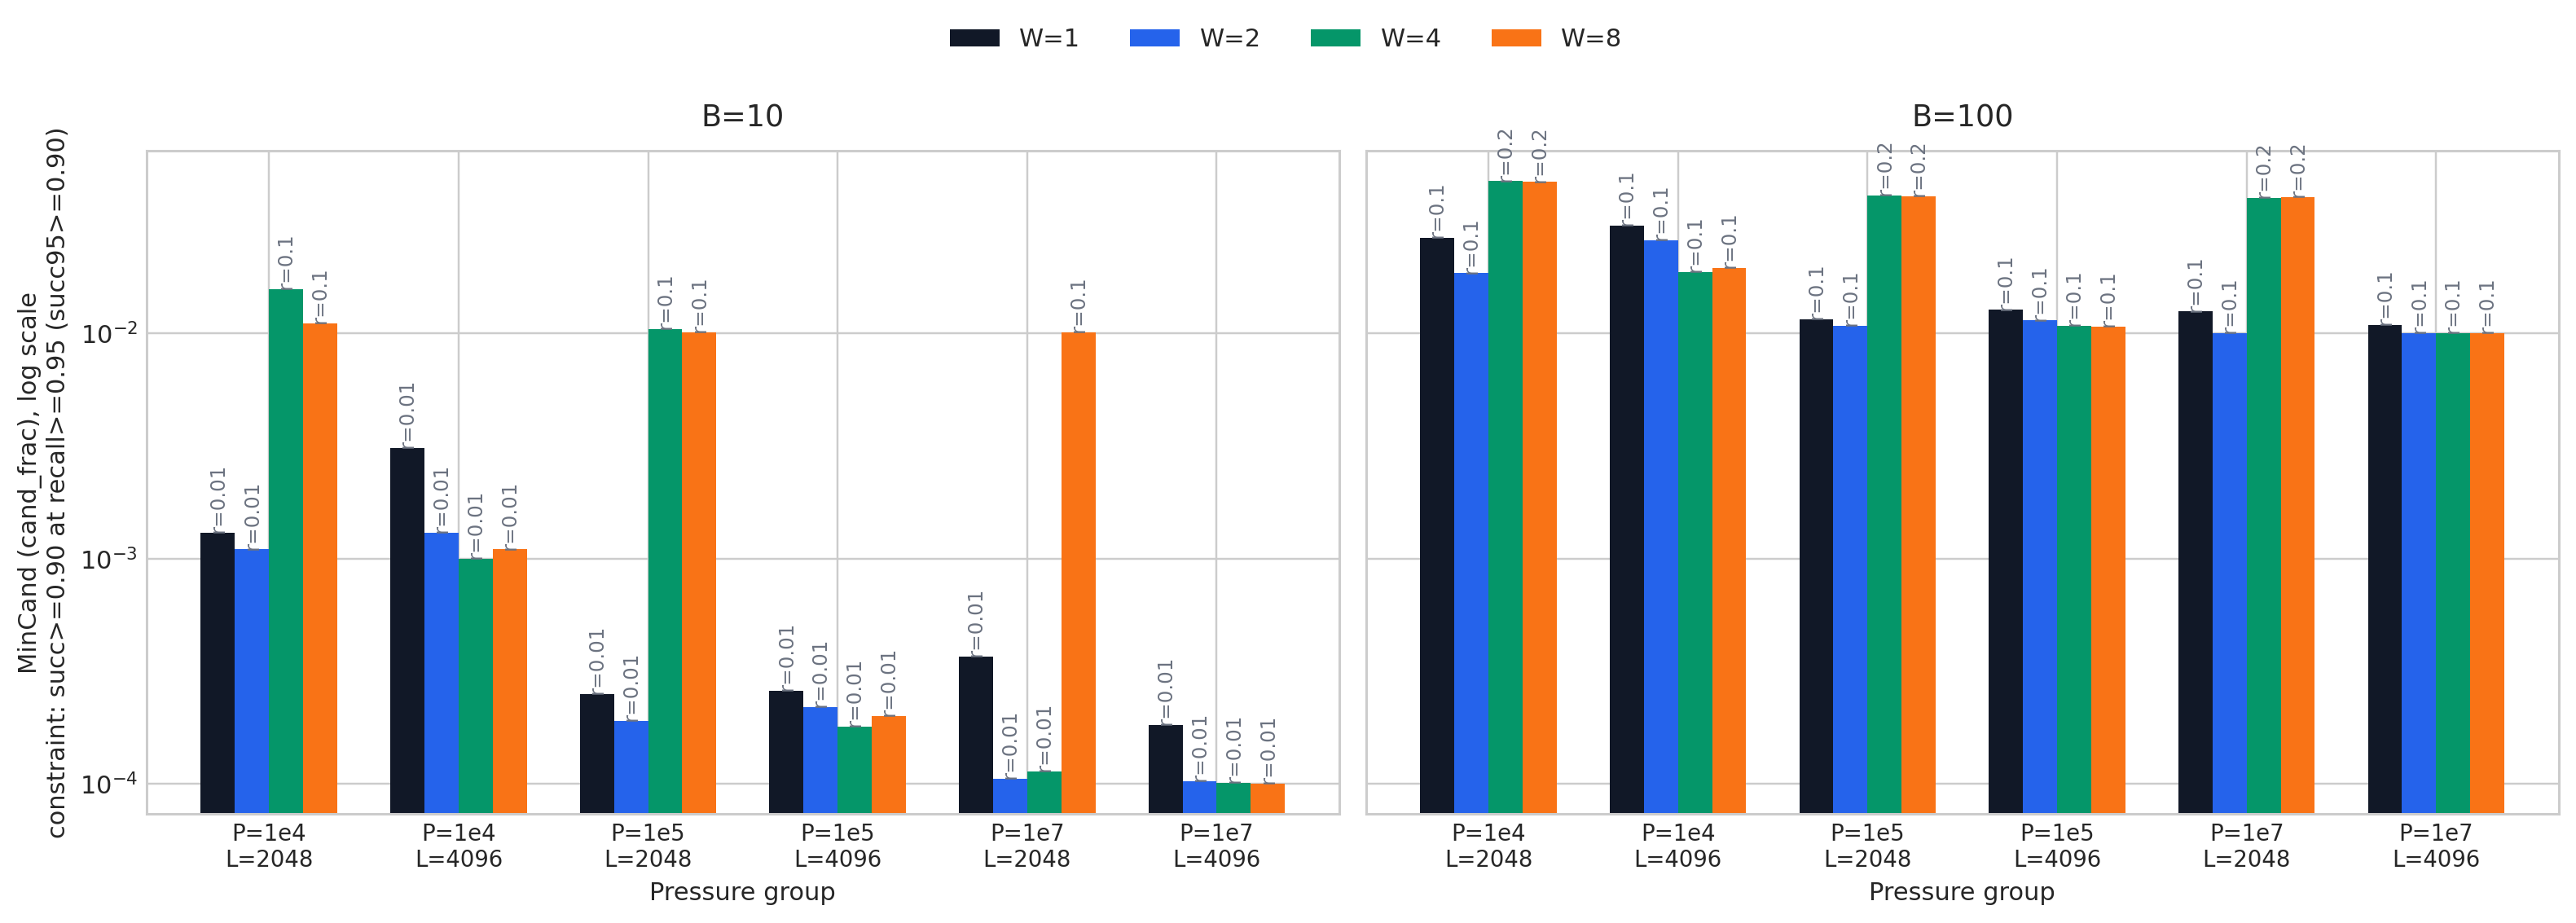
\includegraphics[width=0.9\textwidth]{figures/fig_mincand_by_W_pressure_modern2.png}
\caption{Window-width $W$ ablation: minimum \texttt{cand\_frac} required to meet the reliability threshold across pressure configurations (log scale; lower is better).}
\label{fig:c1-2}
\end{figure*}




This section provides the full configuration and results for the $W$ ablation experiment described in \S\ref{sec:eval-spatial}.

We sweep $W \in \{1,2,4,8,L\}$ under the configurations in Table~\ref{tab:c1-1}, where $W=L$ serves as a negative control in which spatial locality is entirely destroyed.

\begin{table}[!htbp]
\centering
\small
\begin{tabular}{ll}
\toprule
Parameter & Values \\
\midrule
$W$ & $\{1, 2, 4, 8, L\}$ \\
$(P, L)$ & $\{(10^4, 2048), \ldots, (10^7, 4096)\}$ \\
$B$ & $\{10, 100\}$ \\
Fixed & $V=2,\ k=3,\ m_0=32$, strategy \texttt{window\_topr} \\
\bottomrule
\end{tabular}
\caption{Ablation configuration for window width $W$ (fixed $V{=}2,\ k{=}3,\ m_0{=}32$, strategy \texttt{window\_topr}).}
\label{tab:c1-1}
\end{table}



Figure~\ref{fig:c1-2} summarizes the sweep of the minimum \texttt{cand\_frac} across pressure configurations for $W \in \{1,2,4,8\}$. To make the trend concrete, Table~\ref{tab:c1-2} reports representative $B{=}10$ configurations and the corresponding savings of $W{=}2$ over $W{=}1$. Across these settings, a modest contiguous window ($W{=}2$) consistently matches or improves upon per-section ranking ($W{=}1$), and the gain becomes more pronounced as collision pressure $P/L$ increases. At the highest-pressure point ($P{=}10^7$, $L{=}2048$), $W{=}2$ reduces candidate cost by approximately $3.8\times$ relative to $W{=}1$. The benefit does not grow monotonically with $W$, however: when dirty windows already occupy a dense portion of the section axis, the compression of the operating top-$r$ quota is no longer sufficient to offset the larger halo induced by wider windows, and reversal appears in dense low-$L/B$ settings. Table~\ref{tab:c1-w-full} reports the full numerical values, and Supplement~\ref{sec:appendix-w-pricing} analyzes the underlying trade-off.

\begin{table}[!thbp]
\centering
\small
\begin{tabular}{llll}
\toprule
Pressure & \shortstack{$W=1$\\\texttt{cand\_frac}} & \shortstack{$W=2$\\\texttt{cand\_frac}} & \shortstack{$W=2$ vs.\\ $W=1$ saving} \\
\midrule
$P=10^4, L=2048$ & 0.0013 & 0.0010 & 1.3$\times$ \\
$P=10^5, L=2048$ & 0.000245 & 0.000215 & 1.1$\times$ \\
$P=10^7, L=2048$ & 0.000397 & 0.000105 & \textbf{3.8$\times$} \\
$P=10^7, L=4096$ & 0.000176 & 0.000104 & \textbf{1.8$\times$} \\
\bottomrule
\end{tabular}
\caption{Minimum \texttt{cand\_frac} under symmetric injection ($B=10$, fixed $V{=}2,\ k{=}3,\ m_0{=}32$).}
\label{tab:c1-2}
\end{table}

Figure~\ref{fig:c1-1} isolates the negative-control boundary case $W{=}L$. Once the window spans the entire section axis, all segments share the same global window and spatial locality disappears. The reverse-mapped candidate set therefore degenerates toward the full segment universe, yielding $\texttt{cand\_cnt}\approx P$ in the boundary regime. This behavior confirms that candidate compression depends on preserving locality on the section axis, rather than merely increasing the number of covered sections.





Table~\ref{tab:c1-w-full} reports the full numerical values. For $B=10$, the benefit of $W>1$ is more pronounced at high collision pressure, whereas for $B=100$ the differences among $W$ values narrow considerably.

\begin{table}[!thbp]
\centering
\small
\setlength{\tabcolsep}{3pt}
\begin{tabular}{@{}rrcccc@{}}
\toprule
$P$ & $L$ & $W=1$ & $W=2$ & $W=4$ & $W=8$ \\
\midrule
\multicolumn{6}{l}{\textbf{$B=10$}}\\
$10^4$ & 2048 & 0.0013 & 0.0011 & 0.0157 & 0.0111 \\
$10^4$ & 4096 & 0.0031 & 0.0013 & 0.0010 & 0.0011 \\
$10^5$ & 2048 & 0.00025 & 0.00019 & 0.01045 & 0.0101 \\
$10^5$ & 4096 & 0.00026 & 0.00022 & 0.00018 & 0.0002 \\
$10^7$ & 2048 & 0.0003674 & 0.0001054 & 0.0001137 & 0.0100871 \\
$10^7$ & 4096 & 0.0001832 & 0.0001029 & 0.0001012 & 0.0001005 \\
\midrule
\multicolumn{6}{l}{\textbf{$B=100$}}\\
$10^4$ & 2048 & 0.0266 & 0.0185 & 0.0474 & 0.0470 \\
$10^4$ & 4096 & 0.0301 & 0.0259 & 0.0187 & 0.0195 \\
$10^5$ & 2048 & 0.01152 & 0.01079 & 0.04097 & 0.04066 \\
$10^5$ & 4096 & 0.01271 & 0.01141 & 0.01081 & 0.01073 \\
$10^7$ & 2048 & 0.0125068 & 0.0100346 & 0.0400252 & 0.0401635 \\
$10^7$ & 4096 & 0.0108632 & 0.0100551 & 0.010038 & 0.0100062 \\
\bottomrule
\end{tabular}
\caption{Minimum \texttt{cand\_frac} for $W\in\{1,2,4,8\}$ under two density levels ($B\in\{10,100\}$).}
\label{tab:c1-w-full}
\end{table}

For a more intuitive comparison of the relative performance of each $W$ value across configurations, Figure~\ref{fig:c1-3} presents a pairwise dominance-rate heatmap: each cell indicates the fraction of all pressure points at which the row method achieves a lower \texttt{cand\_frac} than the column method.

\begin{figure}[!htbp]
\centering
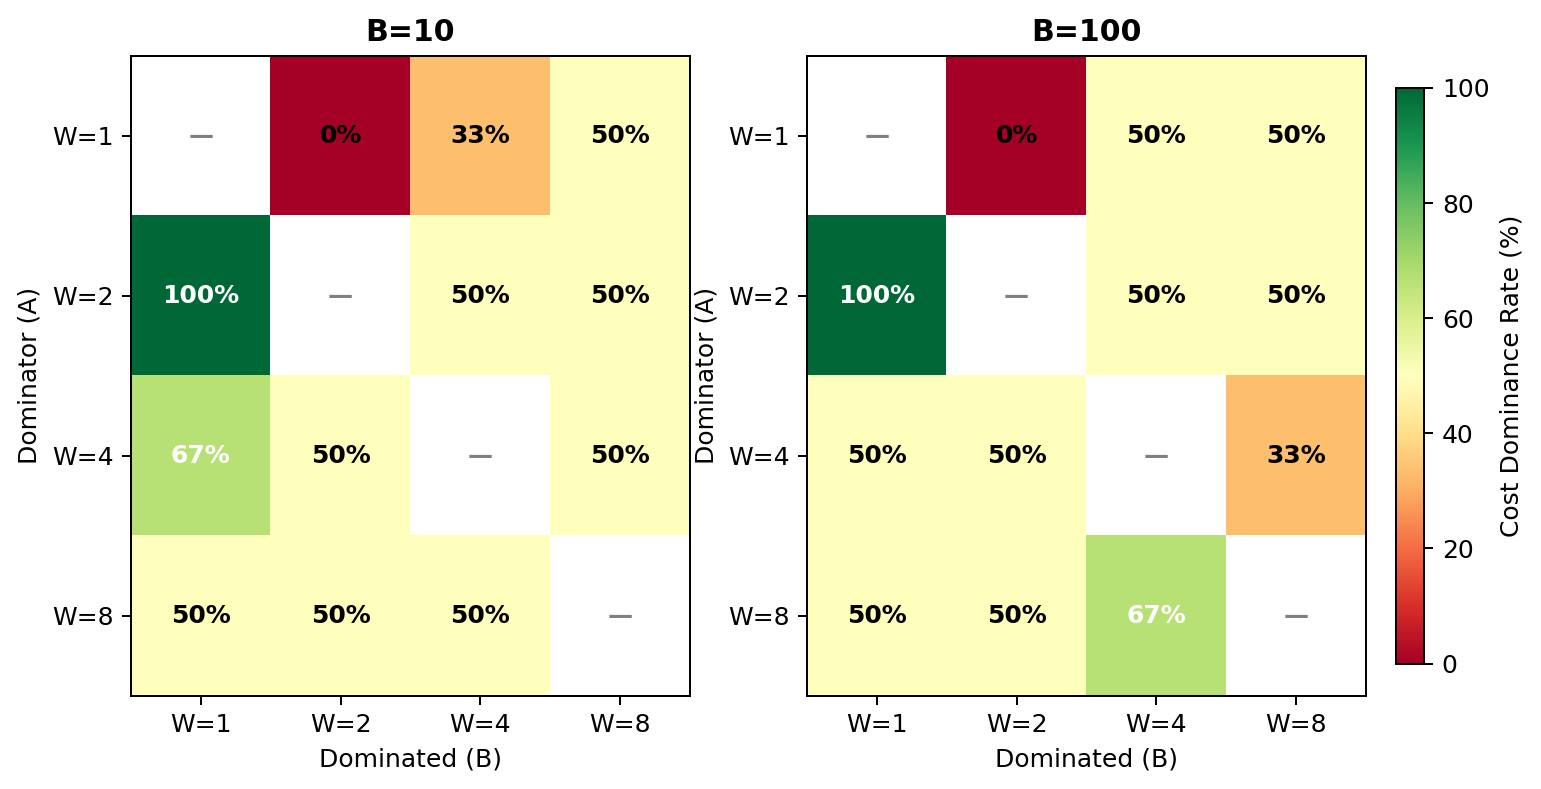
\includegraphics[width=0.95\linewidth]{figures/fig_dominance_heatmap.png}
\caption{Pairwise dominance-rate heatmap across pressure configurations. Cell $(i,j)$ shows the fraction of all pressure points at which $W=i$ achieves a lower minimum \texttt{cand\_frac} than $W=j$ (ties count as $0.5$). Greener cells indicate that the row $W$ wins more frequently.}
\label{fig:c1-3}
\end{figure}

\begin{figure*}[!thbp]
\centering
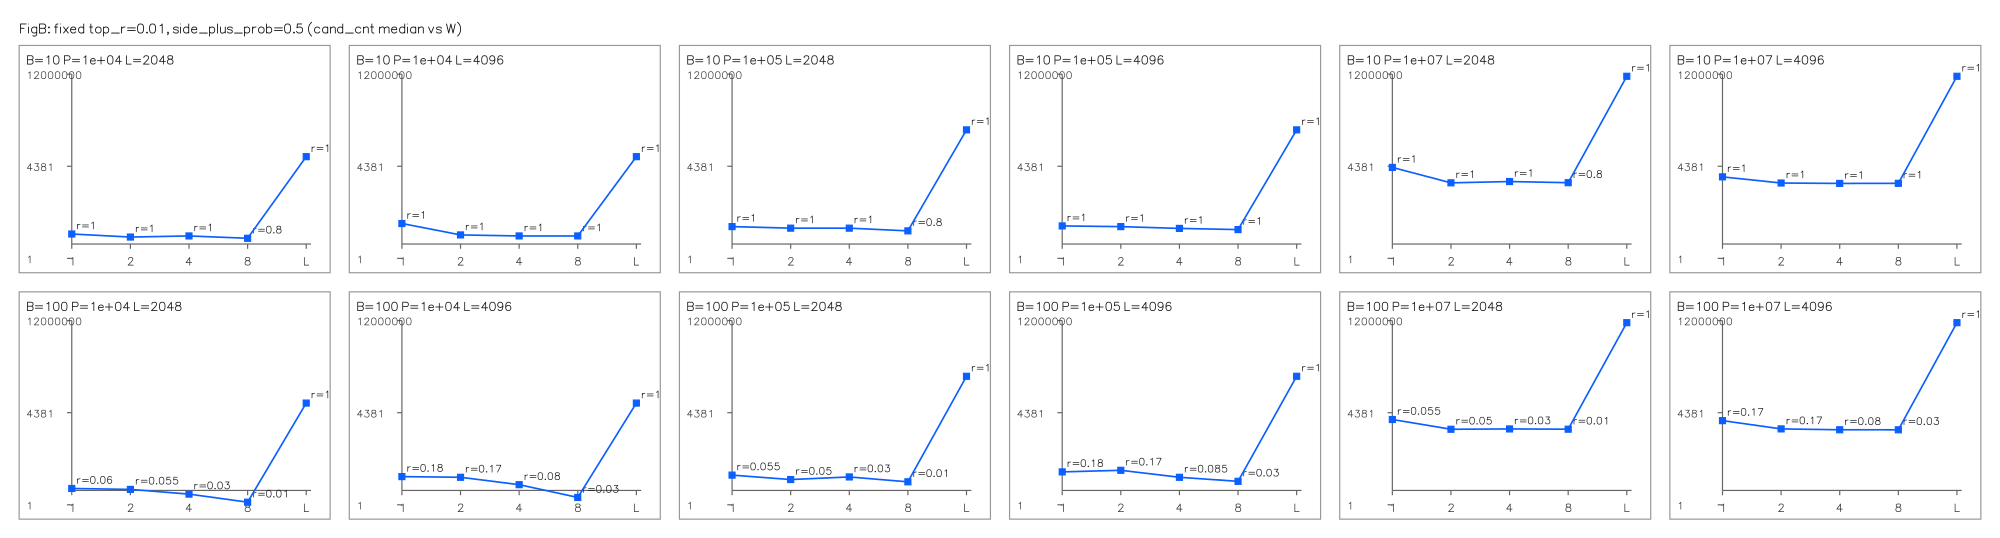
\includegraphics[width=0.9\linewidth]{figures/figB_fixed_topr001_cand_cnt_vs_W.png}
\caption{Absolute candidate count $\texttt{cand\_cnt}$ as a function of $W$ under a fixed truncation budget ($\texttt{top\_r}{=}0.01$). The rightmost point in each curve corresponds to $W{=}L$ (negative control).}
\label{fig:c1-1}
\end{figure*}

\subsection{Energy Signal Coverage Verification}

Figure~\ref{fig:c1-4} in the main text demonstrates the advantage of contiguous structure (\texttt{WindowStart}) over random grouping (\texttt{RandomSections}) through diff-capture curves. This section complements that comparison with energy signal coverage curves, verifying from the perspective of observable quantities whether ``high-energy regions are more concentrated''---the intermediate mechanism. Figure~\ref{fig:c1-5} shows that under \texttt{WindowStart}, selecting the top-$r$ fraction of high-energy regions captures a larger share of total energy; this corroborates the diff-capture curves in the main text.

\begin{figure}[!htbp]
\centering
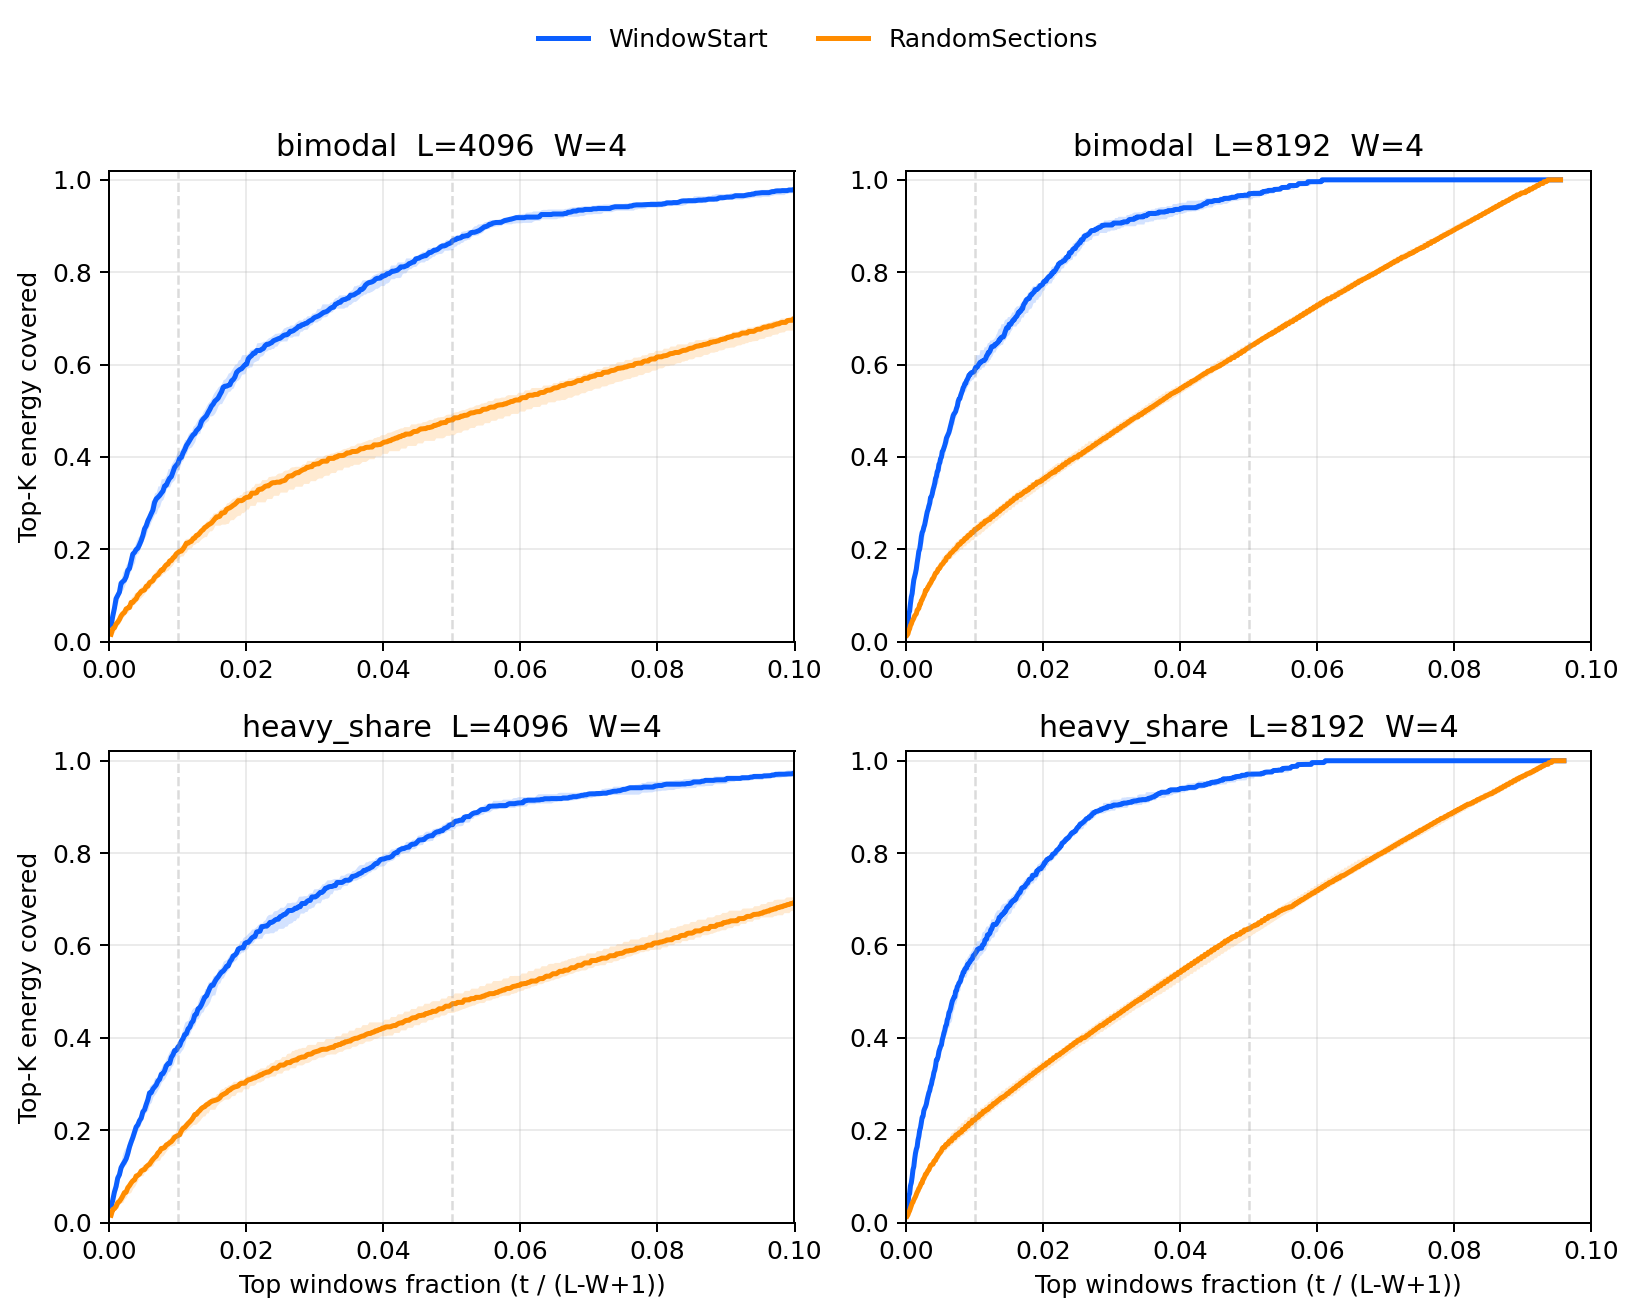
\includegraphics[width=0.95\linewidth]{figures/fig_topk_projected_window_coverage_energy.png}
\caption{Top-$K$ energy coverage. x-axis: top-$r$; y-axis: cumulative energy share. The \texttt{WindowStart} curve is steeper.}
\label{fig:c1-5}
\end{figure}

\subsection{Halo Suppression via Cold-Zone Signals}
\label{sec:appendix-halo}


Following the definition in the main text, $\texttt{halo}=\texttt{cand\_frac}\cdot(P/B)$ represents the candidate multiplier---the factor by which the candidate set exceeds the $B$ dirty segments that must be covered. Under the reliability threshold ($\texttt{succ95} \geq 0.90$, meaning at least 95\% recall in at least 90\% of trials), we select the minimum candidate budget that achieves the target recall and take the more conservative result across the two sides.

%Table~\ref{tab:c1-a2} compares the four strategies at the representative density level $B=100$, and Table~\ref{tab:c1-a3} shows how the best strategy behaves as dirty-segment density varies from $B=10$ to $B=100$. The analysis below uses these tables to examine both the halo suppression effect of each strategy and its sensitivity to dirty-segment density.

\paragraph{Strategy comparison}

\begin{table}[!htbp]
\centering
\small
\begin{tabular}{lcc}
\toprule
Strategy & Halo factor & Relative to baseline \\
\midrule
\texttt{section\_topr} & \textbf{22.0$\times$} & (baseline) \\
\texttt{window\_topr} & 4.2$\times$ & 5.2$\times$ better \\
\texttt{hotcold\_r} & 16.4$\times$ & 1.3$\times$ better \\
\texttt{window\_topr\_hotcold} & \textbf{4.0$\times$} & \textbf{5.5$\times$ better} \\
\bottomrule
\end{tabular}
\caption{$B=100$: best operating-point comparison (same budget; under reliability constraint).}
\label{tab:c1-a2}
\end{table}

Table~\ref{tab:c1-a2} presents the best operating-point comparison across strategies under the same budget framework at $B=100$. The combined strategy \texttt{window\_topr\_hotcold} reduces the halo to $4.0\times$, a roughly $5.5\times$ improvement over the baseline that does not exploit contiguity (\texttt{section\_topr}, $22.0\times$). Additionally, \texttt{hotcold\_r} alone ($16.4\times$) performs far worse than the combination with window-based localization, indicating that cold-zone signals are better suited as a second-stage filter after contiguous-window localization, rather than as a standalone first-stage localization mechanism.

\begin{table}[!htbp]
\centering
\small
\begin{tabular}{rll}
\toprule
$B$ & Best strategy & \texttt{halo} (interpretation) \\
\midrule
10 & \texttt{window\_topr\_hotcold} & \shortstack[l]{\textbf{1.0}  (candidate size \\ on the order of $B$)} \\
100 & \texttt{window\_topr\_hotcold} & \shortstack[l]{\textbf{4.0}  (still better \\ than baseline's 22)} \\
\bottomrule
\end{tabular}
\caption{Representative halo values as dirty-segment density varies.}
\label{tab:c1-a3}
\end{table}


\paragraph{Halo variation with dirty-segment density}

Table~\ref{tab:c1-a3} shows the halo level of the best strategy under two density levels. When dirty segments are sparse ($B=10$), \texttt{window\_topr\_hotcold} achieves a halo of approximately $1.0$, meaning the candidate-set size is of the same order as the number of truly dirty segments and downstream verification incurs virtually no extra overhead. When dirty segments are denser ($B=100$), the halo rises to approximately $4.0$, consistent with the increased overlap of energy peaks on the section axis and higher collision pressure. Nonetheless, the combined strategy remains significantly better than all alternatives at both density levels. This reduction in halo cost under the combined strategy is consistent with the controlled candidate behavior observed in \S\ref{sec:eval-operating}.
